% LNCS format — CENG 467 Final Report
% Erman Akıncı · Ahmet Yılmaz · Kaan Cesur
% İzmir Institute of Technology, Spring 2026

\documentclass{llncs}

\usepackage[utf8]{inputenc}
\usepackage[T1]{fontenc}
\usepackage[a4paper, top=25mm, bottom=25mm, left=25mm, right=25mm]{geometry}
\usepackage{graphicx}
\usepackage{booktabs}
\usepackage{amsmath}
\usepackage{url}
\usepackage{microtype}
\usepackage[hidelinks]{hyperref}
\usepackage{tikz}
\usetikzlibrary{arrows.meta, shapes.geometric, positioning, fit, backgrounds}

\begin{document}

\title{Advanced RAG with Hard Negative Mining for\\Multi-Hop Question Answering}

\author{
    Erman Ak\i nc\i \and
    Ahmet Y\i lmaz \and
    Kaan Cesur
}

\institute{
    \"{I}zmir Institute of Technology (\"{I}YTE), \"{I}zmir, Turkey \\
    \email{\{300201066, 300201067, 290201066\}@std.iyte.edu.tr}
}

\maketitle

% ---------------------------------------------------------------
\begin{abstract}
Retrieval-Augmented Generation (RAG) systems ground language model outputs
in retrieved evidence, reducing hallucination in open-domain question
answering. A critical bottleneck is the retriever: dense retrievers require
hard negative training examples to distinguish superficially similar but
factually incorrect passages. We build a complete RAG pipeline on HotpotQA,
training a Dense Passage Retrieval (DPR) model with BM25-mined hard
negatives, indexing passages in a FAISS vector database, and integrating
Flan-T5-xl as a generative reader. Hard negative mining improves Recall@1
by 13.0 percentage points over vanilla DPR (0.844 vs.\ 0.714) and by 14.0
points over BM25 (0.704), with consistent gains in MRR@10 (0.895 vs.\ 0.793)
and nDCG@10 (0.811 vs.\ 0.688 for vanilla DPR). End-to-end evaluation with Flan-T5-xl achieves
F1\,=\,0.583 and Exact Match\,=\,0.466. An ablation study over three retrieval
configurations shows that the pretrained (Natural Questions) DPR does not
consistently outperform the lexical BM25 baseline --- it leads marginally
at R@1 but falls behind at R@3, R@5, and R@10 --- and that the decisive
improvement is driven entirely by hard negative fine-tuning, and is
statistically significant ($p < 0.001$, paired bootstrap). A per-category
breakdown identifies bridge (multi-hop) questions as the dominant remaining
failure mode, while yes/no questions are handled well.
\keywords{Retrieval-Augmented Generation \and Dense Passage Retrieval \and
Hard Negative Mining \and Multi-Hop Question Answering \and HotpotQA}
\end{abstract}

% ---------------------------------------------------------------
\section{Introduction}

Large language models (LLMs) are prone to hallucination when answering
factual questions from parametric memory alone~\cite{lewis2020rag}.
Retrieval-Augmented Generation (RAG) addresses this by conditioning answer
generation on passages retrieved from an external corpus, grounding outputs
in verifiable evidence. The retrieval component is a critical bottleneck:
if the retriever fails to surface the correct passage, no reader can
recover the correct response regardless of its quality.

Classical lexical retrievers such as BM25~\cite{robertson2009bm25} fail on
paraphrased or semantically complex queries. Dense Passage
Retrieval~\cite{karpukhin2020dpr} overcomes this by learning semantic
representations via bi-encoder models, but requires carefully constructed
training data. Randomly sampled negatives provide insufficient gradient
signal~\cite{xiong2021ance}; hard negative mining selects passages that
score highly on a retrieval metric yet do not contain the gold answer,
forcing the retriever to learn fine-grained semantic distinctions.

Multi-hop question answering tasks such as HotpotQA~\cite{yang2018hotpotqa}
require combining evidence from two supporting passages, making them
especially sensitive to retrieval quality. In this paper we: (1) mine hard
negatives using BM25, (2) fine-tune DPR with a contrastive objective, (3)
index all passages in a FAISS vector database, and (4) integrate
Flan-T5-xl~\cite{chung2022flant5} as a generative reader. We conduct a
systematic ablation study and provide a qualitative error analysis of
failure cases.

% ---------------------------------------------------------------
\section{Related Work}

Karpukhin et al.~\cite{karpukhin2020dpr} introduced DPR, a bi-encoder
model matching questions and passages via dot-product similarity. Trained
with in-batch negatives on Natural Questions, DPR substantially outperformed
BM25 and established the foundation for dense retrieval. Our work extends
this architecture with domain-specific hard negatives on HotpotQA.

Xiong et al.~\cite{xiong2021ance} formalised negative quality in contrastive
training through ANCE, which refreshes hard negatives from the retriever's
own top results at each checkpoint. Their analysis demonstrated that random
negatives produce trivially separable training signal. We adopt their core
insight using BM25-retrieved passages as hard negatives --- a computationally
cheaper alternative that ANCE itself showed to be competitive with
retriever-based mining.

Qu et al.~\cite{qu2021rocketqa} further improved dense retrieval through
cross-encoder-filtered hard negatives in RocketQA, achieving
state-of-the-art retrieval and providing an upper bound for hard negative
training. Lewis et al.~\cite{lewis2020rag} proposed the RAG framework
motivating our pipeline, showing that grounding generation in retrieved
passages substantially reduces hallucination. Yang et
al.~\cite{yang2018hotpotqa} introduced HotpotQA, which requires aggregating
evidence from two supporting passages and has become the standard multi-hop
reasoning benchmark. Khattab and Zaharia~\cite{khattab2020colbert} proposed
ColBERT's late-interaction retrieval, which achieves higher accuracy than
standard bi-encoders at the cost of larger index size and serves as a
reference for understanding retrieval quality trade-offs.
Izacard and Grave~\cite{izacard2021fid} introduced Fusion-in-Decoder (FiD),
which encodes retrieved passages independently with a T5 encoder and fuses
them in the decoder, directly motivating our choice of a generative reader
that can synthesise information across multiple passages. Our Flan-T5-xl
reader follows the same encode-and-generate paradigm without requiring
task-specific reader fine-tuning.

% ---------------------------------------------------------------
\section{System Overview}

Figure~\ref{fig:pipeline} illustrates the end-to-end pipeline. Hard
negative mining and DPR fine-tuning occur offline; the context encoder is
also used offline to encode all corpus passages and build the FAISS index.
At inference time, only the question encoder, the pre-built FAISS index,
and the Flan-T5-xl reader are active.

\begin{figure}[t]
\centering
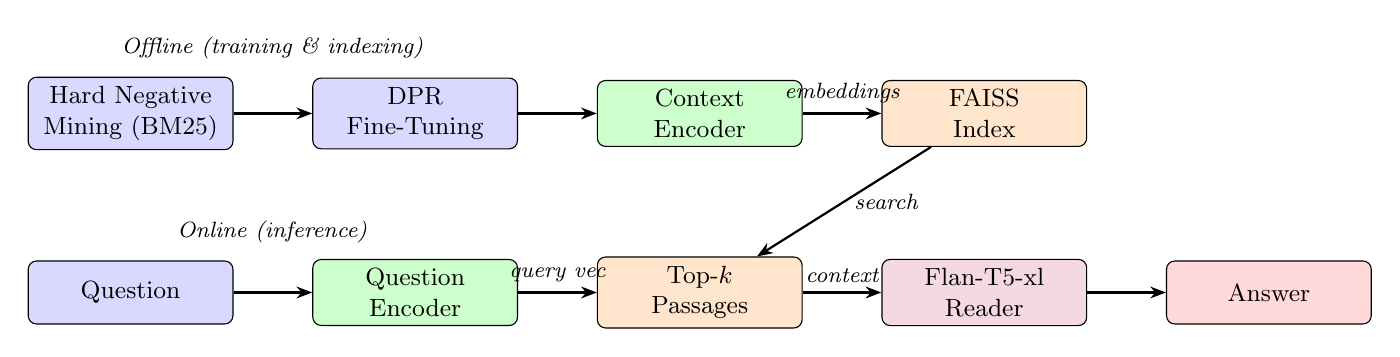
\begin{tikzpicture}[
    node distance = 6mm and 10mm,
    box/.style  = {draw, rounded corners=3pt, fill=#1, minimum width=26mm,
                   minimum height=8mm, align=center, font=\small},
    arr/.style  = {-{Stealth[length=2mm]}, thick},
    lbl/.style  = {font=\footnotesize\itshape},
]
% Offline path (top row)
\node[box=blue!15]  (hn)  {Hard Negative\\Mining (BM25)};
\node[box=blue!15, right=of hn] (train) {DPR\\Fine-Tuning};
\node[box=green!20, right=of train] (ctx)  {Context\\Encoder};
\node[box=orange!20, right=of ctx]  (faiss){FAISS\\Index};

\draw[arr] (hn)    -- (train);
\draw[arr] (train) -- (ctx);
\draw[arr] (ctx)   -- node[above,lbl]{embeddings} (faiss);

% Online path (bottom row)
\node[box=blue!15, below=14mm of hn]  (q)    {Question};
\node[box=green!20, right=of q]        (qenc) {Question\\Encoder};
\node[box=orange!20, right=of qenc]    (ret)  {Top-$k$\\Passages};
\node[box=purple!15, right=of ret]     (rd)   {Flan-T5-xl\\Reader};
\node[box=red!15,    right=of rd]      (ans)  {Answer};

\draw[arr] (q)    -- (qenc);
\draw[arr] (qenc) -- node[above,lbl]{query vec} (ret);
\draw[arr] (faiss) -- node[right,lbl]{search} (ret);
\draw[arr] (ret)  -- node[above,lbl]{context} (rd);
\draw[arr] (rd)   -- (ans);

% Labels
\node[lbl, above=1mm of hn,  xshift=18mm] {Offline (training \& indexing)};
\node[lbl, above=1mm of q,   xshift=18mm] {Online (inference)};

\end{tikzpicture}
\caption{End-to-end RAG pipeline. The offline stage mines hard negatives
with BM25, fine-tunes DPR, and uses the context encoder to build a FAISS
index over the corpus. At inference, the question encoder retrieves top-$k$
passages which Flan-T5-xl reads to generate the final answer.}
\label{fig:pipeline}
\end{figure}

% ---------------------------------------------------------------
\section{Methodology}

\subsection{Hard Negative Mining}

For each training question $q_i$ with gold passage set $\mathcal{G}_i$,
we run BM25 over the 10 candidate passages and select passages that score
highly but do not belong to the gold supporting facts:
$\mathcal{H}_i = \{ p \in \mathcal{P} \setminus \mathcal{G}_i \mid
\mathrm{rank}_\mathrm{BM25}(p, q_i) \leq K \}$,
with $K = 5$. These hard negatives are lexically similar to the question,
making them genuinely difficult to distinguish from true supporting passages.
In practice, each question yields \emph{at most} 5 hard negatives: examples
for which no gold passage can be identified are discarded, and the available
distractor pool may be smaller than $K$ for some questions. We mine 30{,}000
examples from the HotpotQA train split; after discarding unanswerable
examples and reserving 20\% as a held-out diagnostic set, approximately
24{,}000 examples remain for training.

\subsection{DPR Fine-Tuning}

We fine-tune the pretrained DPR question and context encoders
(\texttt{facebook/dpr-*-single-nq-base}) with contrastive loss. For a
mini-batch of size $B$, each question's positive passage is placed on the
diagonal of the similarity matrix; all remaining in-batch positives
\emph{together with all hard negatives} serve as negatives. Concretely,
the passage matrix $\mathbf{P}$ has $B + B \cdot n_\mathrm{HN}$ rows, where
$n_\mathrm{HN}$ is the number of hard negatives per question in the current
epoch:
\begin{equation}
    \mathcal{L} = -\frac{1}{B} \sum_{i=1}^{B}
    \log \frac{\exp\!\left(f(q_i)^\top f(p^+_i)\right)}
         {\displaystyle\sum_{j=1}^{B + B \cdot n_\mathrm{HN}}
          \exp\!\left(f(q_i)^\top f(p_j)\right)}
\end{equation}
where $f(\cdot)$ is the encoder's pooler output (768 dimensions) and the
denominator ranges over all $B$ positives plus $B \cdot n_\mathrm{HN}$
hard negatives concatenated in the batch. We use AdamW with
$lr = 2\times10^{-5}$, gradient clipping (max\_norm\,=\,1.0), and a linear
LR scheduler with 10\% warmup steps to stabilise contrastive training. We
apply a \textbf{curriculum strategy}: epoch~1 uses 1 hard negative per
question, epoch~2 uses 3, and epoch~3 uses the full 5. This prevents early
gradient instability caused by excessively difficult negatives at the start
of training. We checkpoint every epoch and select the final model by
\textbf{global-corpus retrieval} on the ablation set, not by the per-question
mini-pool used during training: with only the $\sim$7 in-batch candidates per
question, the mini-pool metric saturates and correlates poorly with
open-corpus retrieval. The final model (\textit{DPR + HN}) is trained on
the full $\sim$24{,}000-example training split with batch size 16.

\subsection{Training Configuration}

Table~\ref{tab:hyperparams} lists the hyperparameters used for DPR
fine-tuning. Training uses in-batch negatives together with curriculum
hard negatives, gradient clipping, and a warmup--decay learning-rate
schedule throughout.

\begin{table}[h]
\centering
\caption{DPR fine-tuning hyperparameters.}
\label{tab:hyperparams}
\begin{tabular}{ll}
\toprule
\textbf{Hyperparameter} & \textbf{Value} \\
\midrule
Base model              & \texttt{facebook/dpr-*-single-nq-base} \\
Optimizer               & AdamW \\
Learning rate           & $2 \times 10^{-5}$ \\
LR scheduler            & Linear warmup (10\%) + linear decay \\
Batch size              & 16 \\
Epochs                  & 3 \\
Max question length     & 64 tokens \\
Max passage length      & 256 tokens \\
Hard negatives/question & Curriculum: 1 $\to$ 3 $\to$ 5 per epoch \\
Gradient clipping       & max\_norm\,=\,1.0 \\
Checkpoint selection    & Best epoch by global-corpus retrieval \\
Hardware                & NVIDIA A100 (40 GB) \\
\bottomrule
\end{tabular}
\end{table}

\subsection{FAISS Vector Index}

All unique passages from the 500 validation examples (approximately 4{,}900
passages after title-based deduplication) are encoded offline with the
context encoder and indexed using FAISS
\texttt{IndexFlatIP}~\cite{johnson2019faiss}, which performs exact
inner-product search. At inference time, the question encoder produces a
query vector and FAISS returns the top-$k$ nearest passages by dot-product
similarity. This global index simulates a realistic retrieval scenario where
the retriever searches a shared corpus rather than the per-question local
pool of 10 candidates, making evaluation significantly harder.

\subsection{Generative Reader}

The top-3 retrieved passages are concatenated (truncated to 2{,}000 characters)
and passed to Flan-T5-xl~\cite{chung2022flant5} (3B parameters) with an
instruction prompt:
\textit{``Answer the question based on the context below. Context: [passages].
Question: [q]. Answer:''}
The model generates the answer with greedy decoding (up to 50 tokens) via
\texttt{model.generate}. We use a generative reader because multi-hop HotpotQA
answers are frequently yes/no responses or short inferential spans that benefit
from synthesising evidence across passages rather than copying a single
contiguous span.

% ---------------------------------------------------------------
\section{Experimental Setup}

We evaluate on the first 500 examples of the HotpotQA distractor validation
split~\cite{yang2018hotpotqa}. Each question has 10 candidate passages (2
gold + 8 distractors). We report \textbf{Recall@k} (fraction of questions for
which at least one gold passage appears in the top-$k$ retrieved passages,
$k \in \{1, 3, 5, 10\}$), \textbf{MRR@10} and \textbf{nDCG@10} (ranking
quality, treating the supporting-fact passages as relevant), \textbf{Token F1}
(token-level overlap after lowercasing and punctuation removal), and
\textbf{Exact Match (EM)} (normalised string equality). The complete codebase
is available at
\url{https://github.com/ahmet-yilmaz-cs/CENG467_Term_Project}.

We compare three configurations under identical conditions (same 500 validation
examples, same global passage corpus of approximately 4{,}900 passages, same
Flan-T5-xl reader). BM25 searches this corpus with \texttt{rank\_bm25}; both
DPR variants build a FAISS index over the same passages:
\textbf{(1) BM25} --- lexical retrieval with \texttt{rank\_bm25};
\textbf{(2) DPR (vanilla)} --- pretrained DPR without fine-tuning;
\textbf{(3) DPR + HN} --- DPR fine-tuned on the hard-negative training split.

% ---------------------------------------------------------------
\section{Results}

\subsection{Ablation Study}

Table~\ref{tab:ablation} reports retrieval quality and Table~\ref{tab:qa} the
end-to-end QA metrics across all three configurations.

\begin{table}[t]
\centering
\caption{Retrieval quality on 500 HotpotQA validation examples over the same
global FAISS corpus. Recall@k is the fraction of questions
with at least one gold passage in the top $k$; MRR@10 and nDCG@10 measure
ranking quality.}
\label{tab:ablation}
\begin{tabular}{lrrrrrr}
\toprule
\textbf{Configuration} & \textbf{R@1} & \textbf{R@3} & \textbf{R@5}
    & \textbf{R@10} & \textbf{MRR@10} & \textbf{nDCG@10} \\
\midrule
BM25                   & 0.704 & 0.862 & 0.904 & 0.980 & 0.793 & 0.692 \\
DPR (vanilla)          & 0.714 & 0.854 & 0.888 & 0.932 & 0.793 & 0.688 \\
DPR + HN               & \textbf{0.844} & \textbf{0.936} & \textbf{0.962}
    & \textbf{0.984} & \textbf{0.895} & \textbf{0.811} \\
\bottomrule
\end{tabular}
\end{table}

\begin{table}[t]
\centering
\caption{End-to-end QA on 500 HotpotQA validation examples (Flan-T5-xl reader
on the top-3 retrieved passages). Better retrieval propagates to higher
answer quality.}
\label{tab:qa}
\begin{tabular}{lrr}
\toprule
\textbf{Configuration} & \textbf{F1} & \textbf{EM} \\
\midrule
BM25                   & 0.496 & 0.388 \\
DPR (vanilla)          & 0.485 & 0.384 \\
DPR + HN               & \textbf{0.583} & \textbf{0.466} \\
\bottomrule
\end{tabular}
\end{table}

\noindent\textbf{Effect of hard negative mining.}
DPR + HN improves Recall@1 by 13.0 percentage points over vanilla DPR
(0.844 vs.\ 0.714) and by 14.0 points over BM25 (0.704). The gains hold at
every cutoff (R@3 +8.2 pp, R@5 +7.4 pp over vanilla) and, crucially, at the top of
the ranking: MRR@10 rises from 0.793 to 0.895 and nDCG@10 from 0.688 to
0.811. Because the reader consumes only the top-3 passages, these
top-of-ranking gains are exactly what propagate to answer quality. The results
confirm that hard negative mining substantially strengthens retrieval by
forcing the model to distinguish semantically similar but factually incorrect
passages.

\noindent\textbf{BM25 vs.\ vanilla DPR.}
The pretrained DPR (Natural Questions) does not consistently outperform the
lexical BM25 baseline: it leads marginally at R@1 (0.714 vs.\ 0.704, a
difference of one percentage point), but falls behind at R@3, R@5, and R@10
(e.g.\ 0.932 vs.\ 0.980 at R@10) and is essentially tied at MRR@10 and
nDCG@10. This pattern is expected --- vanilla DPR has not been adapted to
HotpotQA's multi-hop bridging structure --- and shows that out-of-the-box
dense retrieval does not reliably improve over lexical search. The decisive
advantage appears only after hard negative fine-tuning, which surpasses both
baselines decisively across all metrics.

\subsection{End-to-End QA Performance}

The full pipeline (DPR + HN + FAISS + Flan-T5-xl) achieves F1\,=\,0.583 and
EM\,=\,0.466 (Table~\ref{tab:qa}). The same reader on the vanilla DPR and BM25
retrievers reaches only F1\,=\,0.485 and F1\,=\,0.496 respectively, so the
retrieval gains from hard negative mining translate directly into a $\sim$0.10
F1 and 0.08 EM improvement downstream.

\noindent\textbf{Reader input budget.}
The single largest reader-side lever was the tokeniser input limit. At 512
tokens, the instruction, the 2{,}000-character context, and the question
together exceed the budget and the question is truncated; raising the limit to
1{,}024 tokens recovers roughly 4 F1 points uniformly across all configurations
(DPR + HN: 0.539\,$\to$\,0.583 F1). This was a larger gain than any prompt or
model change we tried.

\noindent\textbf{Reader comparison.}
Table~\ref{tab:readers} compares three readers on the fixed DPR + HN retriever,
each in its best configuration. Flan-T5-xl (3B, encoder--decoder) slightly
outperforms the larger Qwen2.5-7B-Instruct and the smaller
Phi-4-mini-Instruct. Few-shot prompting with answer post-processing helps the
decoder-only instruction model (Qwen: +0.025 F1) but is neutral for the others,
and the long multi-part instruction actually \emph{harms} Flan-T5-xl ---
prompt sensitivity is model-specific. The reader runs zero-shot; its absolute
score is further bounded by multi-hop questions that require synthesising both
supporting passages, analysed next.

\begin{table}[t]
\centering
\caption{Reader comparison on the fixed DPR + HN retriever (top-3 passages,
500 validation questions), each reader in its best configuration. The 7B and
3.8B decoder-only models are 4-bit quantised.}
\label{tab:readers}
\begin{tabular}{lrr}
\toprule
\textbf{Reader} & \textbf{F1} & \textbf{EM} \\
\midrule
Flan-T5-xl (3B)            & \textbf{0.583} & \textbf{0.466} \\
Qwen2.5-7B-Instruct        & 0.574 & 0.452 \\
Phi-4-mini-Instruct (3.8B) & 0.520 & 0.390 \\
\bottomrule
\end{tabular}
\end{table}

\subsection{Statistical Significance and Breakdown}

\noindent\textbf{Significance.}
On the 500 validation questions, DPR + HN improves F1 by $+0.097$ (95\%
bootstrap CI $[+0.061, +0.134]$) and Recall@1 by $+0.130$ ($[+0.086, +0.172]$)
over vanilla DPR; both gains are significant at $p < 0.001$ (paired bootstrap,
5{,}000 resamples). The headline metrics with 95\% CIs are DPR + HN
R@1 $= 0.844\,[0.812, 0.876]$ and F1 $= 0.582\,[0.542, 0.621]$, confirming the
improvements are not artefacts of the sample size.

\noindent\textbf{Strict (both-passage) recall.}
HotpotQA answers depend on \emph{two} supporting passages. Under the stricter
criterion that \emph{both} gold passages appear in the top 5, recall drops
sharply --- DPR + HN $0.962 \to 0.616$, vanilla $0.888 \to 0.462$, BM25
$0.904 \to 0.406$ --- revealing the true difficulty of multi-hop retrieval that
the standard ``at least one gold'' criterion masks. DPR + HN retains the
largest margin (+0.15 over vanilla).

\noindent\textbf{Per-category breakdown.}
Table~\ref{tab:breakdown} breaks DPR + HN end-to-end performance down by
question type. Comparison questions (F1 0.781) are handled far better than
bridge questions (F1 0.535), which require following a bridge entity across two
passages and are the dominant failure mode. Yes/no questions, though few
(33/500), are answered nearly perfectly (EM 0.909) --- contrary to the common
assumption that generative readers mishandle them.

\begin{table}[t]
\centering
\caption{DPR + HN end-to-end performance by question category (500 validation
questions; the dev split is entirely ``hard'' level).}
\label{tab:breakdown}
\begin{tabular}{lrrrr}
\toprule
\textbf{Category} & \textbf{n} & \textbf{F1} & \textbf{EM} & \textbf{R@1} \\
\midrule
Bridge      & 404 & 0.535 & 0.416 & 0.817 \\
Comparison  &  96 & 0.781 & 0.677 & 0.958 \\
Yes/no      &  33 & 0.909 & 0.909 & 0.970 \\
Span        & 467 & 0.559 & 0.435 & 0.835 \\
\bottomrule
\end{tabular}
\end{table}

% ---------------------------------------------------------------
\section{Error Analysis}

We inspected failure cases from the DPR + HN pipeline to identify
recurring error patterns, categorising them into retrieval failures (gold
passage not in top-3) and reader failures (gold passage retrieved but answer
wrong).

\paragraph{Retrieval failures --- entity disambiguation.}
The retriever fails on questions that require precise disambiguation of
similarly-named entities. For example:
\begin{quote}
\small
\textit{Q: Who was known by his stage name Aladin and helped organisations
improve their performance as a consultant?} \quad
\textit{Gold answer: Eenasul Fateh}
\end{quote}
BM25 and vanilla DPR both retrieve passages about the fictional character
Aladdin (high lexical overlap with ``Aladin''), missing the passage about
Eenasul Fateh, a Bangladeshi-British artist. DPR + HN correctly surfaces
the gold passage by leveraging semantic context around the consultant
relation, demonstrating the value of hard negative training.

\paragraph{Yes/no questions are handled well.}
Contrary to the common assumption that generative readers mishandle binary
questions, the breakdown (Table~\ref{tab:breakdown}) shows yes/no is in fact the
strongest category (EM 0.909). Occasional formatting slips still occur:
\begin{quote}
\small
\textit{Q: Are the Laleli Mosque and Esma Sultan Mansion in the same
neighbourhood?} \quad
\textit{Gold: no} \quad \textit{Predicted: They are in different
neighbourhoods of Istanbul}
\end{quote}
Here the prediction is semantically correct but fails exact match; such cases
are rare, and a concise-answer instruction largely resolves them.

\paragraph{Multi-hop reasoning failures.}
Some questions require chaining two facts where the connection is implicit:
\begin{quote}
\small
\textit{Q: The director of the romantic comedy ``Big Stone Gap'' is based in
what New York neighbourhood?} \quad
\textit{Gold: Greenwich Village, New York City} \quad
\textit{Predicted: New York City}
\end{quote}
The reader identifies the correct city but omits the specific neighbourhood,
yielding partial F1 and EM\,=\,0. Quantitatively, bridge questions --- which
require this chaining --- score far below comparison questions (F1 0.535
vs.\ 0.781; Table~\ref{tab:breakdown}), making them the dominant failure mode.

\paragraph{Context truncation failures.}
The reader input is truncated to 2{,}000 characters to fit within the
model's effective context window. For questions whose gold evidence
appears late in the retrieved passages, the truncation discards the
relevant sentences entirely:
\begin{quote}
\small
\textit{Q: Which film has the director born first, ``All Roads Lead to Rome''
or ``Amreeka''?} \quad
\textit{Gold: Amreeka} \quad \textit{Predicted: All Roads Lead to Rome}
\end{quote}
The passage containing the director's birth year for \textit{Amreeka}
falls beyond the 2{,}000-character cutoff, causing the reader to generate
an answer based on incomplete evidence. Increasing the context budget
(e.g., using a longer-context reader such as Flan-T5-xl with extended
positional encoding) would directly address this failure mode.

% ---------------------------------------------------------------
\section{Discussion}

\paragraph{Hard negative mining is the decisive factor.}
The jump from vanilla DPR (R@1 0.714, roughly on par with BM25 at 0.704) to
DPR + HN (R@1 0.844) validates our core hypothesis: the gain comes from
domain-specific hard negatives, not from dense retrieval per se. Training on
the full $\sim$24{,}000-example split with gradient clipping, a warmup--decay
schedule, and curriculum hard negatives is stable and improves monotonically
across epochs, with no sign of degradation at scale.

\paragraph{Checkpoint selection must match the evaluation setting.}
During training we score checkpoints on the per-question mini-pool
($\sim$7 candidates: the positives plus their hard negatives), but this metric
saturates and does not track open-corpus quality. Selecting the final epoch on
the global corpus instead is what reliably identifies the best
model; relying on the mini-pool metric can select a checkpoint that looks
strong locally yet retrieves poorly at corpus scale. This also explains the
gap between a near-saturated training-time Recall@5 and the global-corpus
Recall@5\,=\,0.962 reported here --- the two measure fundamentally different
retrieval difficulties.

\paragraph{Reader limitations.}
The Flan-T5-xl reader runs zero-shot. The dominant remaining failure mode is
bridge (multi-hop) questions (F1 0.535 vs.\ 0.781 for comparison), followed by
context truncation; yes/no and comparison questions are already handled well.
A stronger or fine-tuned reader and a larger context budget would partially
address the remaining cases.

% ---------------------------------------------------------------
\section{Ethical Considerations}

\paragraph{Hallucination risk.}
Flan-T5-xl is a generative model and may produce answers not grounded in
retrieved passages. We mitigate this by constraining input to retrieved
evidence and using greedy decoding; however, the model can still
hallucinate when retrieved passages are insufficient or misleading.

\paragraph{Coverage bias.}
HotpotQA is derived from Wikipedia, which overrepresents English-language
and Western-centric content. Retrieval and reading performance is expected
to be lower on questions about underrepresented topics or named entities
with limited Wikipedia coverage.

\paragraph{Evaluation limitations.}
Token F1 and Exact Match against a single reference answer penalise
semantically correct paraphrases. For yes/no questions, a model generating
a correct explanatory sentence receives partial F1 credit despite being
factually correct, distorting aggregate evaluation.

% ---------------------------------------------------------------
\section{Conclusion}

We presented a complete RAG pipeline for multi-hop question answering
combining BM25-based hard negative mining, DPR fine-tuning, FAISS vector
indexing, and Flan-T5-xl generative reading. Hard negative mining improves
Recall@1 by 13.0 points over vanilla DPR and 14.0 points over BM25, with
matching gains in MRR@10 and nDCG@10, and these retrieval gains carry through
to the end-to-end QA metrics (F1\,=\,0.583, EM\,=\,0.466). Our ablation shows
that out-of-the-box dense retrieval does not consistently outperform BM25 on
this multi-hop benchmark --- leading only marginally at R@1 while falling
behind at higher cutoffs --- and that the improvement is attributable entirely
to hard negative fine-tuning. Selecting checkpoints on the global corpus
rather than a small per-question pool is essential for a faithful comparison.
Future work should scale hard negative mining to the full 90k training split,
fine-tune the reader, and evaluate over a full open-domain Wikipedia corpus
for an even more realistic retrieval scenario.

% ---------------------------------------------------------------
\begin{thebibliography}{9}

\bibitem{karpukhin2020dpr}
Karpukhin, V., Oguz, B., Min, S., Lewis, P., Wu, L., Edunov, S., Chen, D.,
Yih, W.: Dense passage retrieval for open-domain question answering.
In: Proceedings of EMNLP, pp. 6769--6781 (2020)

\bibitem{xiong2021ance}
Xiong, L., Xiong, C., Li, Y., Tang, K.F., Liu, J., Bennett, P., Ahmed, J.,
Overwijk, A.: Approximate nearest neighbor negative contrastive learning
for dense text retrieval. In: Proceedings of ICLR (2021)

\bibitem{qu2021rocketqa}
Qu, Y., et al.: RocketQA: An optimized training approach to dense passage
retrieval for open-domain question answering.
In: Proceedings of NAACL, pp. 5835--5847 (2021)

\bibitem{lewis2020rag}
Lewis, P., et al.: Retrieval-augmented generation for knowledge-intensive
NLP tasks. In: Proceedings of NeurIPS, pp. 9459--9474 (2020)

\bibitem{yang2018hotpotqa}
Yang, Z., et al.: HotpotQA: A dataset for diverse, explainable multi-hop
question answering. In: Proceedings of EMNLP, pp. 2369--2380 (2018)

\bibitem{khattab2020colbert}
Khattab, O., Zaharia, M.: ColBERT: Efficient and effective passage search
via contextualized late interaction over BERT.
In: Proceedings of SIGIR, pp. 39--48 (2020)

\bibitem{robertson2009bm25}
Robertson, S., Zaragoza, H.: The probabilistic relevance framework: BM25
and beyond. Foundations and Trends in Information Retrieval 3(4),
333--389 (2009)

\bibitem{johnson2019faiss}
Johnson, J., Douze, M., J{\'e}gou, H.: Billion-scale similarity search
with GPUs. IEEE Transactions on Big Data 7(3), 535--547 (2021)

\bibitem{chung2022flant5}
Chung, H.W., et al.: Scaling instruction-finetuned language models.
arXiv:2210.11416 (2022)

\bibitem{izacard2021fid}
Izacard, G., Grave, E.: Leveraging passage retrieval with generative
models for open domain question answering.
In: Proceedings of EACL, pp. 874--880 (2021)

\end{thebibliography}

\end{document}
